
\begin{example}
Περιγράψτε το μετασχηματισμό $M_L$, που βρίσκεται το συμμετρικό ενός αντικειμένου ως προς μία ευθεία $L$, που τέμνει τον άξονα των $y$ στο $(0,b)$ και σχηματίζει με τον άξονα των $x$ γωνία $\theta$.
\end{example}
\begin{solution}



Εφαρμόζουμε γεωμετρικούς μετασχηματισμούς. Θα προσπαθήσουμε να ανάγουμε το ζητούμενο μετασχηματισμό σε σύνθεση βασικών μετασχηματισμών και ιδιαίτερα της βασικής συμμετρίας ως προς τους άξονες $x$ και $y$. Εκτελούμε τα ακόλουθα βήματα:


Βήμα 1:  Μεταφέρουμε το σημείο $(0, b)$ στην αρχή των αξόνων. Η μεταφορά θα γίνει κατά διάνυσμα $-v$, όπου $v = b\hat{i}$, $\hat{i}$, $\hat{j}$ τα μοναδιαία στους άξονες $x$ και $y$ αντίστοιχα.

\[
\text{Βασικός πίνακας μετασχηματισμού: } T_{-v}
\]

\begin{figure}[h!]
	\begin{center}

		    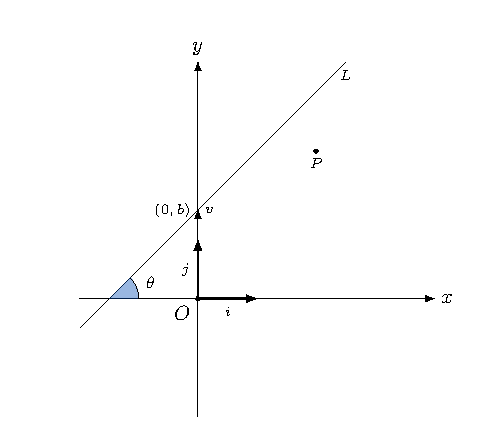
\includegraphics[scale=1]{Chapter2/figure16a.pdf}

	\end{center}
	\caption{πίνακας μετασχηματισμού \textcolor{red}{what}}
\end{figure}

Βήμα 2: Στρέφουμε κατά γωνία $-\theta$ ώστε η ευθεία $L$ να ευθυγραμμιστεί με τον άξονα των $x$.

\[
\text{Βασικός πίνακας μετασχηματισμού: } R_{-\theta}
\]

\begin{figure}[h!]
	\begin{center}

		    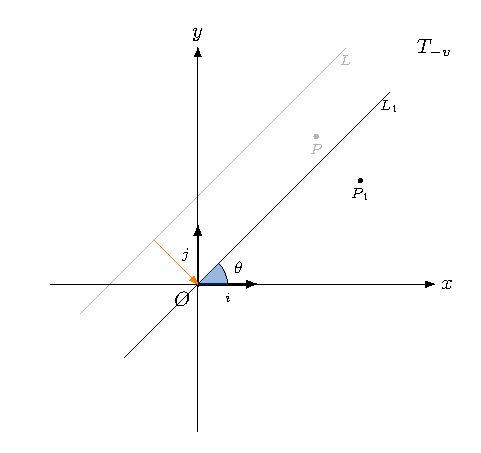
\includegraphics[scale=1]{Chapter2/figure16b.pdf}
	\end{center}
	\caption{πίνακας μετασχηματισμού \textcolor{red}{what}}
\end{figure}

Βήμα 3: Παίρνουμε το συμμετρικό ως προς τον άξονα των $x$.

\[
\text{Βασικός πίνακας μετασχηματισμού: } M_x
\]

\begin{figure}[h!]
	\begin{center}

		    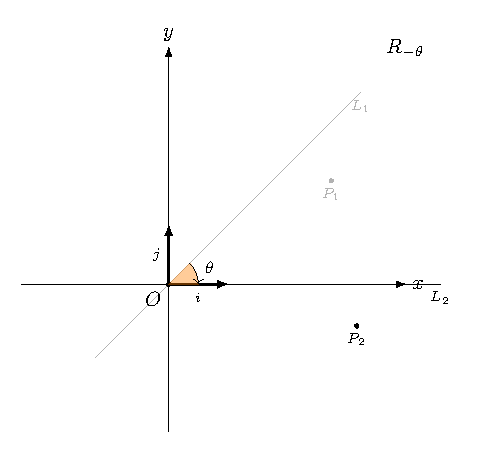
\includegraphics[scale=1]{Chapter2/figure16c.pdf}

	\end{center}
	\caption{πίνακας μετασχηματισμού \textcolor{red}{what}}
\end{figure}

Βήμα 4: Εκτελούμε στροφή κατά γωνία $\theta$.

\[
\text{Βασικός πίνακας μετασχηματισμού: } R_\theta
\]

\begin{figure}[h!]
	\begin{center}

		    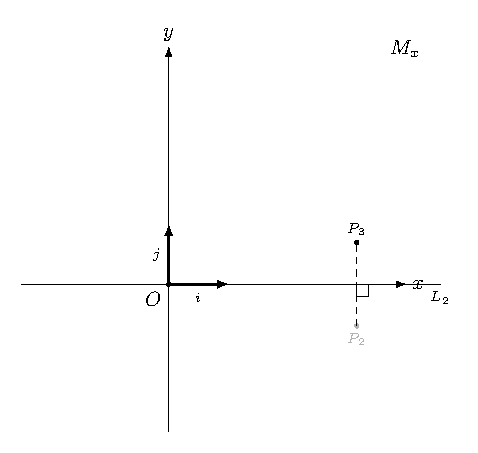
\includegraphics[scale=1]{Chapter2/figure16d.pdf}

	\end{center}
	\caption{πίνακας μετασχηματισμού \textcolor{red}{what}}
\end{figure}


Βήμα 5: \textcolor{red}{Συμμετρικό} ως προς άξονα $x$.

\[
\text{Βασικός πίνακας μετασχηματισμού: } M_x
\]


\begin{figure}[h!]
	\begin{center}

		    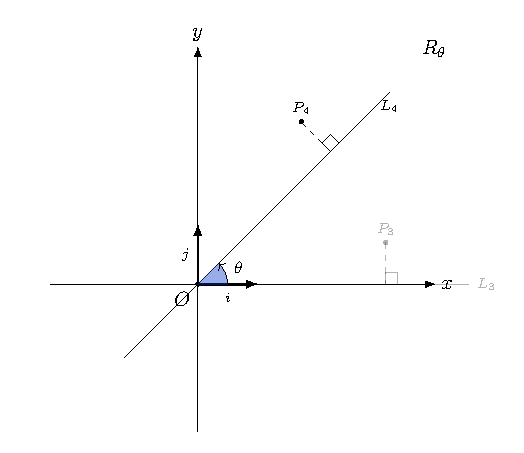
\includegraphics[scale=1]{Chapter2/figure16e.pdf}

	\end{center}
	\caption{πίνακας μετασχηματισμού \textcolor{red}{what}}
\end{figure}


Βήμα 6: Επαναφέρουμε το σημείο $(O, b)$ στην αρχική του θέση. Η μεταφορά θα γίνει κατά διάνυσμα $v$.


\[
\text{Βασικός πίνακας μετασχηματισμού: } T_v
\]

\begin{figure}[h!]
	\begin{center}

		    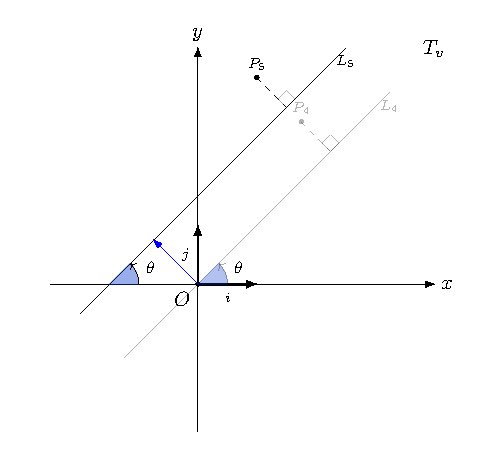
\includegraphics[scale=1]{Chapter2/figure16f.pdf}

	\end{center}
	\caption{πίνακας μετασχηματισμού \textcolor{red}{what}}
\end{figure}

Ο ζητούμενος μετασχηματισμός θα προκύψει σαν σύνθεση των παραπάνω βασικών μετασχηματισμών.

\[
M_L = T_v \cdot R_{\theta} \cdot M_x \cdot R_{-\theta} \cdot T_{-v} \tag{1}
\]

Εάν τώρα υποθέσουμε ότι η κλίση της ευθείας $L$ είναι $m$, δηλαδή $\tan\theta = m$, και κατά συνέπεια $\sin\theta = \cfrac{m}{\sqrt{m^2+1}}$, $\cos\theta = \cfrac{1}{\sqrt{m^2+1}}$, η σχέση (1) γίνεται:

\[
M_L = \begin{bmatrix}
1 & 0 & 0 \\
0 & 1 & b \\
0 & 0 & 1
\end{bmatrix}
\begin{bmatrix}
\cos\theta & -\sin\theta & 0 \\
\sin\theta & \cos\theta & 0 \\
0 & 0 & 1
\end{bmatrix}
\begin{bmatrix}
1 & 0 & 0 \\
0 & -1 & 0 \\
0 & 0 & 1
\end{bmatrix}
\begin{bmatrix}
\cos\theta & \sin\theta & 0 \\
-\sin\theta & \cos\theta & 0 \\
0 & 0 & 1
\end{bmatrix}
\begin{bmatrix}
1 & 0 & 0 \\
0 & 1 & -b \\
0 & 0 & 1
\end{bmatrix}
\]

Με υπολογισμούς προκύπτει:

\[
M_L = \begin{bmatrix}
\cfrac{1 - m^2}{m^2 + 1} & \cfrac{2m}{m^2 + 1} & \cfrac{-2bm}{m^2 + 1} \\
\cfrac{2m}{m^2 + 1} & \cfrac{m^2 - 1}{m^2 + 1} & \cfrac{2b}{m^2 + 1} \\
0 & 0 & 1
\end{bmatrix}
\]
\end{solution}